\documentclass{IEEEcsmag}

\usepackage[colorlinks,urlcolor=blue,linkcolor=blue,citecolor=blue]{hyperref}
\expandafter\def\expandafter\UrlBreaks\expandafter{\UrlBreaks\do\/\do\*\do\-\do\~\do\'\do\"\do\-}
\usepackage{upmath,color}

\usepackage[spanish]{babel}
%\usepackage[latin1]{inputenc}
\usepackage[utf8]{inputenc}  

\jvol{1}
\jnum{1}
\paper{1}
\jmonth{Noviembre}
\jname{ITICs letters}
\jtitle{Proyectos Integradores}
\pubyear{2023}

\newtheorem{theorem}{Theorem}
\newtheorem{lemma}{Lemma}



\setcounter{secnumdepth}{0}

\begin{document}

\sptitle{Proyecto Integrador de Primer Semestre}

\title{Software de resolución de problemas de Ingeniería }

\author {Azael Manuel Otero Reyes }
\affil{Instituto Tecnológico Superior del Occidente del Estado de Hidalgo, Mixquiahuala, Hgo., 42700, Mexico}

\author{Rosario Reyes Martinez }
\affil{Instituto Tecnológico Superior del Occidente del Estado de Hidalgo, Mixquiahuala, Hgo., 42700, Mexico}

%No me aparecia la l asi que solo puse mi segundo nombre
\author{ Aislinn Leilany Sanchez Reyes }
\affil{Instituto Tecnológico Superior del Occidente del Estado de Hidalgo, Mixquiahuala, Hgo., 42700, Mexico}


%\author{Third Author III}
%\affil{Institute, City, (State), Postal Code, Country}

\markboth{ITSOEH/ITICS/PROYECTO INTEGRADOR PRIMER SEMESTRE}{THEME/FEATURE/DEPARTMENT}

\begin{abstract}
This proyect start whit work distribute (in this team is 5 clasmates), estarted for the 
problems, everyone did a problema and we all put together the work to check that the 
procedure was correct.
After that, we start whit the Project, as a team we did and cheked that the steps to follow, 
time passed, the Works were gethered, the Project was made and independently 
participated together to achieve our integrative Project.
Este archivo esta disponible en:
\url{https://github.com/23Leilany166/Integrador_proyecto} para más información.
\end{abstract}
\maketitle


\chapteri{L}a importancia de los manuscritos recae en la función que tienen de transmitir relatos o
conocimientos. A partir de la problemática, “resolución de problemas de ingeniería con software” Se
realizo la investigación de los problemas asignados, al grupo de primer semestre, considerados para
el proyecto integrador. Dando como resultado la codificación de los problemas en lenguaje Java.
Donde se trataron de pulir, los aspectos que debe de tener un profesionista en esta área, de ente los
cuales, los más destacados son: la capacidad para diseñar y realizar proyectos, habilidad para hacer
uso de las nuevas tecnologías conocimientos avanzados en matemáticas, y computación.
Las Tecnologías en Información y Comunicación están presentes en todo el mundo moderno, y han
ayudado a resolver varios problemas en el mundo. Los profesionistas en esta área, deben tener la
capacidad de resolver problemas con las herramientas de vanguardia.
El siguiente manuscrito, tiene como propósito, mostrar a un público en general, como los próximos
profesionistas en TIC’s usan las herramientas y su razonamiento para resolver problemas de Calculo y
Matemáticas Discretas mediante el método de las 6D’s : descripción del problema, definición de la
solución, diseño de la solución, desarrollo de la solución, depuración y pruebas y documentación.
La resolución incluye la codificación de estos problemas, obteniendo como resultado el poder hacer
conversiones entre sistemas binarios a decimales y viceversa. También se podrá dar solución a una
ecuación cuadrática la cual regresará valores de sus raíces en casi de que estén en el conjunto de los
números reales.


\section{PROBLEMAS}
A continuación la resolucion de los problemas.

\begin{enumerate}
\item \subsection{Problema 1}
%Asael Manuel Otero Reyes
    Definir el problema: \\
    - Encontrar la ecuación de la recta que pasa por dos puntos ($A \mbox{ y } B$) y calcular el ángulo entre la recta y el eje horizontal. \\
    Describir el problema: \\
    - Necesitamos desarrollar un programa en Java que tome las coordenadas de dos puntos, A ($x_{1}, y_{1}$) y B ( $x_{2}, y_{2}$), y devuelva la ecuación de la recta (en la forma y = mx + b) y el ángulo en grados entre la recta resultante y el eje horizontal. \\
    Descomponer el problema: \\
    - Subproblema 1: Calcular la ecuación de la recta. \\
    - Calcular la pendiente (m) utilizando la fórmula: `($y_{2}$ - $y_{1}$) / ($x_{2}$ - $x_{1}$)`. \\
    - Calcular la ordenada al origen (b) utilizando la fórmula: `y = mx + b`. \\
    
    - Subproblema 2: Calcular el ángulo entre la recta y el eje horizontal. \\
    - Utilizar la función `Math.atan(pendiente)` para obtener el ángulo en radianes.\\
    - Convertir el ángulo a grados usando `Math.toDegrees()`.\\
    
    \begin{figure}
    \centerline {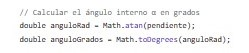
\includegraphics[width=18.5pc]{./latex_imagenes/Img_ejer1_1.jpg}}
    \end{figure}
    
    Desarrollar una solución: \\
    - Solicitar al usuario las coordenadas de los puntos A y B. \\
    - Calcular la pendiente y la ordenada al origen. \\
    - Calcular el ángulo en radianes y convertirlo a grados. \\
    - Imprimir la ecuación de la recta y el ángulo resultante. \\

    Desplegar el plan de acción:
    - Implementar un programa en Java que siga los pasos mencionados.\\
    - Tomar las coordenadas de los puntos A y B como entrada.\\

    - Realizar los cálculos necesarios para obtener la ecuación de la recta y el ángulo. \\

    %Aqui inserten sus imagenes 
    %\begin{figure}
    %\centerline {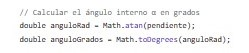
\includegraphics[width=18.5pc]{./latex_imagenes/Img_ejer1_1.jpg}}
    %\end{figure} 

   - Mostrar los resultados al usuario. \\
   %Aqui inserten sus imagenes 
    %\begin{figure}
    %\centerline {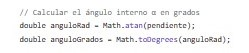
\includegraphics[width=18.5pc]{./latex_imagenes/Img_ejer1_1.jpg}}
    %\end{figure} 

    Depurar y verificar: \\
    - Ejecutar el programa con varios conjuntos de puntos conocidos y verificar que la ecuación de la recta y el ángulo resultantes sean correctos. \\
    - Comprobar cómo maneja el programa casos especiales, como cuando la pendiente es infinita.

\item \subsection{Problema 2}

%Leilany Aislinn Sanchez Reyes

    Descripción del problema: \\
    -Dada una ecuación cuadrática  regresar los valores de las raíces y en caso de que estén sobre los números reales , en caso contrario indicar que la solución está dentro del conjunto de los números complejos.

    Definición de la solución: \\
    - Lo que nos pide  encontrar  es la  solución  de una ecuación cuadrática y si las raíces  pertenecen a los números reales, o  en caso contrario a los números complejos, estaremos utilizando  la fórmula cuadrática también conocida como la fórmula general para resolver el problema \\

    \begin{figure}
    \centerline {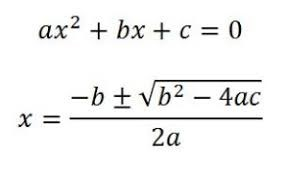
\includegraphics[width=10.5pc]{./latex_imagenes/Img_ejer2_1.jpg}}
    \end{figure}

    Lo primero que voy a definir es el nombre del problema: integrador ejercicio 2 \\
    Después diseñaremos el diagrama de flujo para guiarnos al momento de realizar el código ya que recordemos que los diagramas de flujos son una herramienta  gráfica que nos ayuda a visualizar  la solución para resolver el problema.
        \centering
        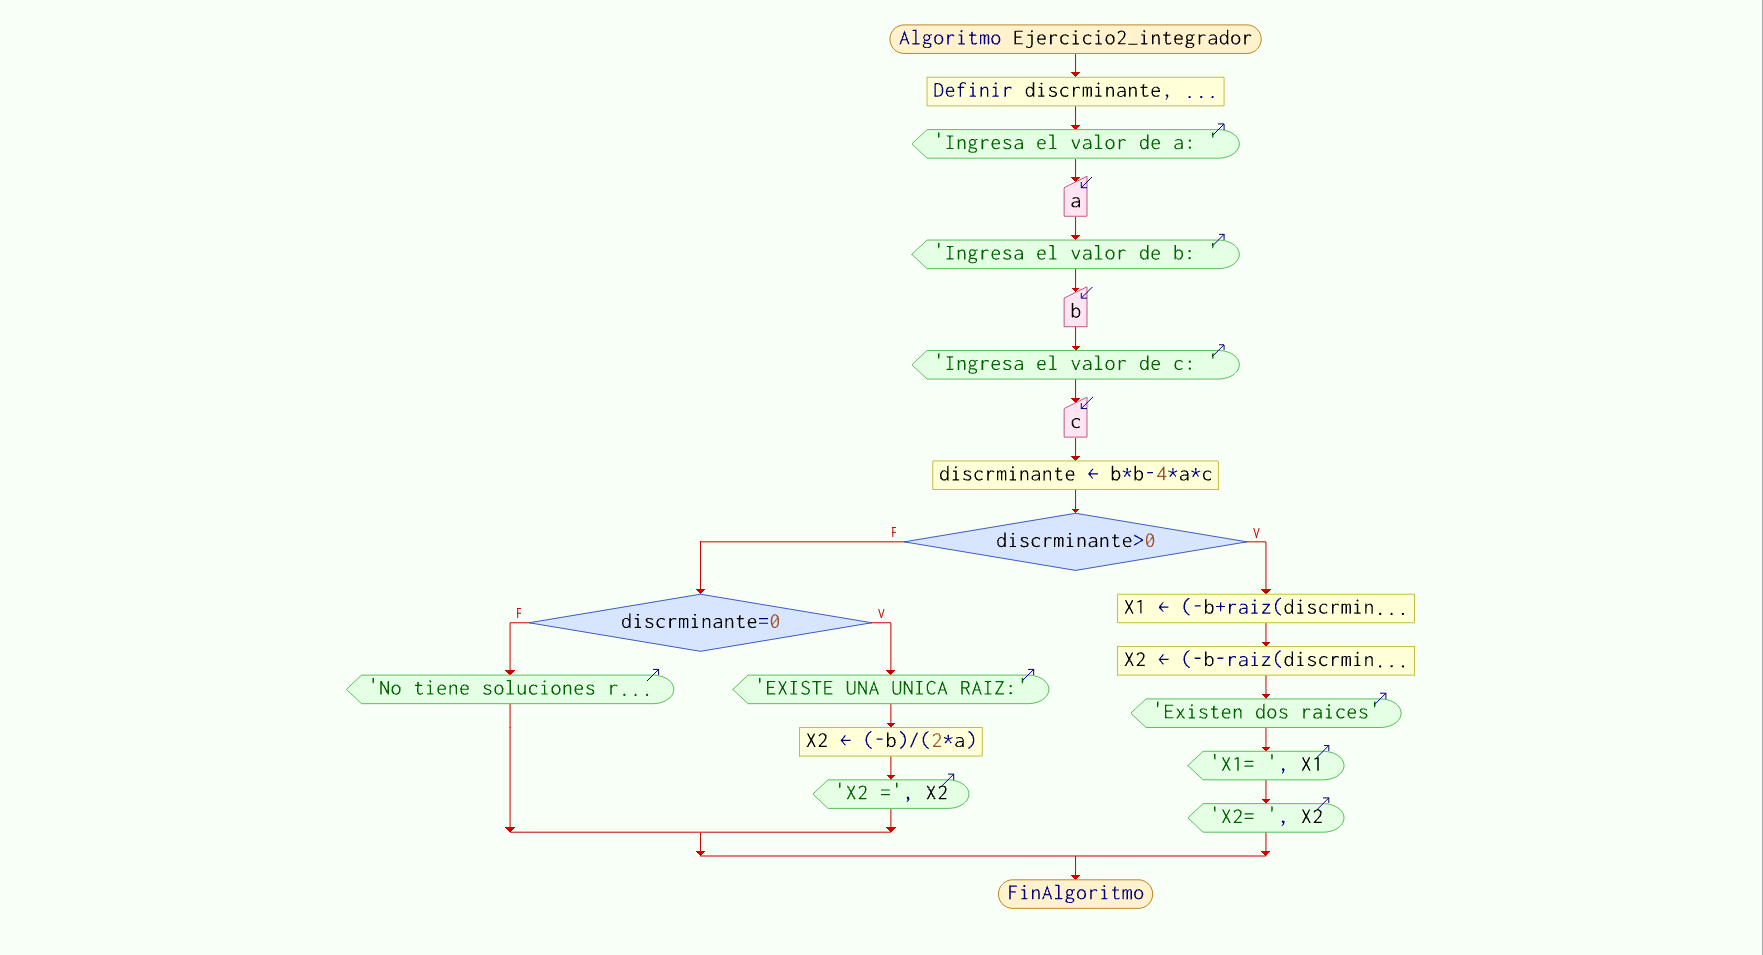
\includegraphics[width=0.5\linewidth]{./latex_imagenes/Diagrama_Integrador.png}
    %\end{figure}
    
    Después lo que  vamos a solicitar son  los valores  de los coeficientes de a,b y c de una ecuación cuadrática y declarar las raíces $x_{1}$ y $x_{2}$.

 
        \centering
        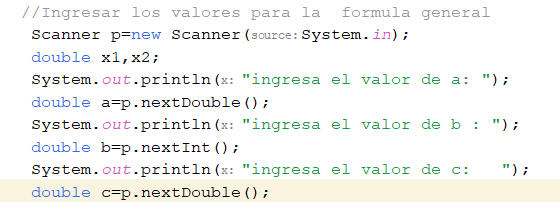
\includegraphics[width=0.5\linewidth]{./latex_imagenes/valores.png}
    %\end{figure}
    
    Después vamos a calcular el discriminante (fórmula general),  con la fórmula  \(b^2 - 4ac\) esta fórmula nos ayudará a determinar el resultado de las raíces.
    
        \centering
        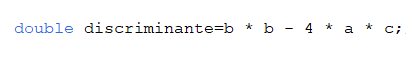
\includegraphics[width=0.5\linewidth]{./latex_imagenes/discrminante.png}
    %\end{figure}
    
    Después el programa verificará el valor  de las raíces  que tiene la evaluación cuadrática $x_{1}$ , $x_{2}$.  entonces vamos a tomar una decisión,  si discriminante>0 va tener dos raíces que son x1,x2 y va a pertenecer a los números reales utilizando la fórmula general que en este caso la variable se nombro discriminante para identificar la formula general.
    
   
        \centering
        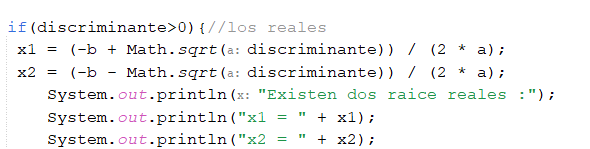
\includegraphics[width=0.5\linewidth]{./latex_imagenes/reales.png}
    %\end{figure}
    
    Después vamos a tomar otra decisión,  si discriminante=0 tiene una sola raíz   en este caso estaremos  utilizando x2 como la raíz .
    
        \centering
        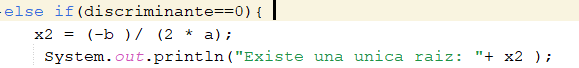
\includegraphics[width=0.5\linewidth]{./latex_imagenes/una raiz.png}
    %\end{figure}

    Y por último si la condición no cumple con ninguna de las dos condiciones el número va a pertenecer a los números complejos
    
        \centering
        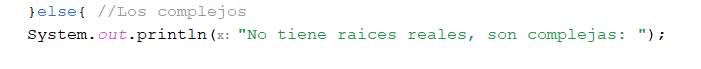
\includegraphics[width=0.5\linewidth]{./latex_imagenes/complejos.png}
    %\end{figure}

    Una vez diseñado el código vamos a realizar una serie de pruebas para ver si la solución de nuestro problema es correcta.\\
    Ejercicios de prueba:
    \begin{align*}
    x^{2} - 2x + 1 &= 0\\
    x^{2} &= 0
    \end{align*}
  
        \centering
        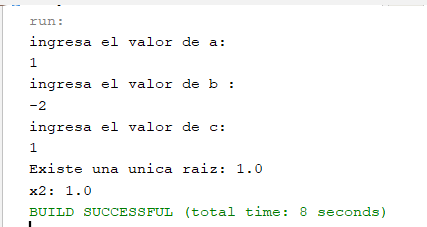
\includegraphics[width=0.5\linewidth]{./latex_imagenes/prueba1.png}
    %\end{figure}
    
    

\item \subsection{Problema 3}
%Rosario Reyes Martinez

    Descripción del Problema:
    - Dada una circunferencia con centro en el punto C con coordenadas ($x_{1}$ , $y_{1}$) y radio r, evaluar si un punto T con coordenadas ($x_{2}$ , $y_{2}$) esta dentro del area de la circunferencia 
    
    Definición de la Solución:
    - Con esto se procede a utilizar la formula para calcular la distancia entre dos puntos, para con esto determinar si el punto T esta dentro de la circunferencia, dependiendo a el radio \\

    \centering
    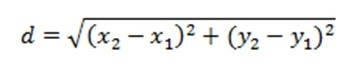
\includegraphics[width=0.5\linewidth]{./latex_imagenes/Img_ejer3_1.jpg}

    Diseño Solución:
    -Partiendo de la definicion se procede a diseñar el diagrama de flujo, el cual permitira un mayor entendimiento al problema planteado 

    \centering
    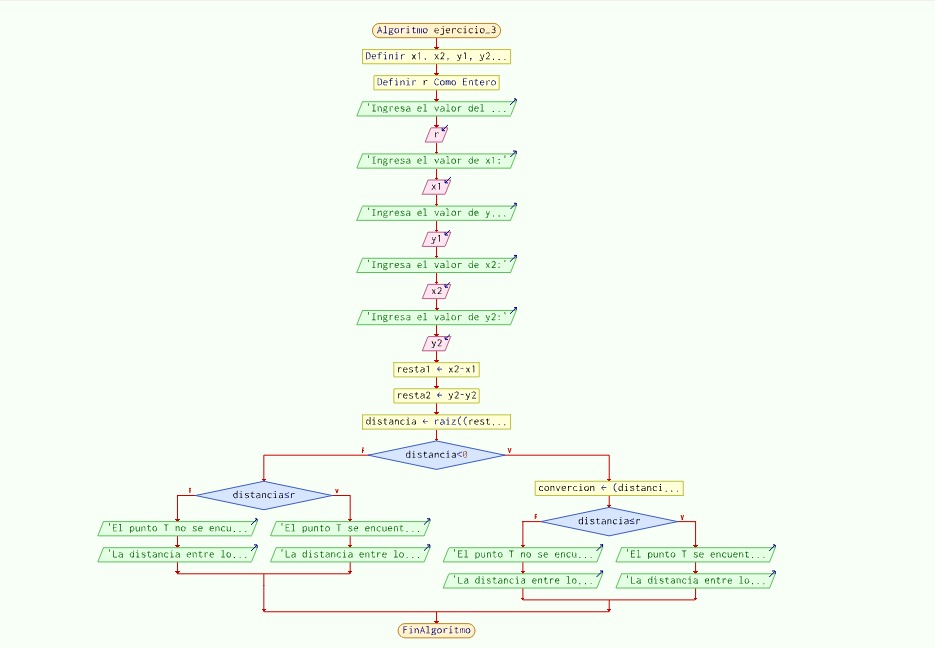
\includegraphics[width=0.5\linewidth]{./latex_imagenes/Img_ejer3_2.jpg}
    
    Desarrollo de Solución:
    - Ahora se comienza la codificacion del problema en el lenguaje de progrmacion java 
    -Declarando las variables como enteros y reales  \\
    \centering
    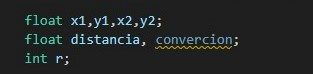
\includegraphics[width=0.5\linewidth]{./latex_imagenes/Img_ejer3_6.jpg}  \\
    -Ingresando los valores que se le daran a las varibles \\
    \centering
    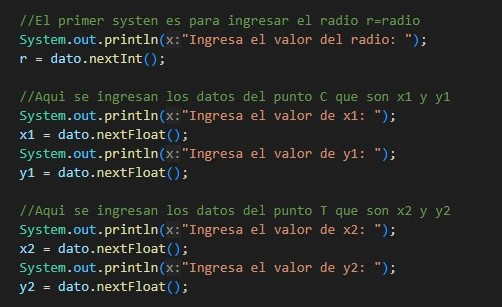
\includegraphics[width=0.5\linewidth]{./latex_imagenes/img_ejer3_4.jpg}  \\
    -Haciendo la operacion para carcular la distancia que hay del punto C, al punto T:
   \centering
    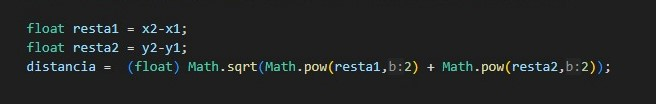
\includegraphics[width=0.5\linewidth]{./latex_imagenes/img_ejer3_3.jpg} \\
    -Para finalmente saber si se encuentra dentro de la circunferencia el punto T o no: \\
    \centering
    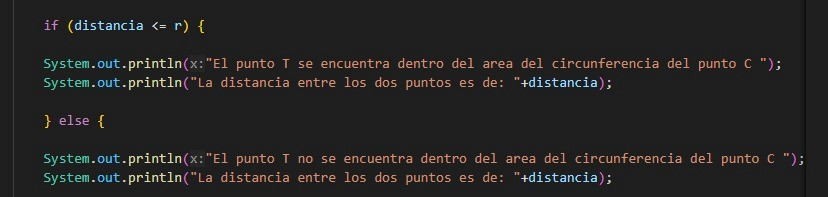
\includegraphics[width=0.5\linewidth]{./latex_imagenes/Img_ejer3_5.jpg}

    Depuración de pruebas:

    Ejemplo:

    \begin{align*}
    (2-2)^{2} + (4-2)^{2} &= 2\\
    radio &= 1\\
    \end{align*}
    El punto T no se encuenta en la circunferencia
   
    \begin{align*}
    (-2-2)^{2} + (4-4)^{2} &= 4\\
    radio &= 5\\
    \end{align*}
    El punto T se encuenta en la circunferencia

\item \subsection{Problema 6}
%Rosario Reyes Martinez

    Descripción del Problema:
    - Dada una tabla de verdad de n bits generar la expresión booleana que genere de manera fidedigna las salidas de esta tabla
    
    Definición de la Solución:
    - Sabiendo esto, se hara el nuestra solucion para un maximo de 4 bits, ya es es con el conocimiento que se cuenta, hasta el momento \\


    Diseño Solución:
    -Partiendo de la definicion se procede a diseñar el diagrama de flujo, el cual permitira un mayor entendimiento al problema planteado 
    
    Desarrollo de Solución:
    - Ahora se comienza la codificacion del problema en el lenguaje de progrmacion java 
    -Ingresando la cantidad de bits, si se pasa de la cantidad definida este imprimira lo que esta fuera de rango \\
    \centering
    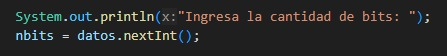
\includegraphics[width=0.5\linewidth]{./latex_imagenes/Img_ejer6_1.jpg}  \\
    \centering
    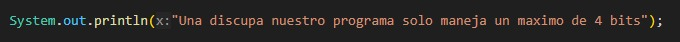
\includegraphics[width=0.5\linewidth]{./latex_imagenes/Img_ejer6_6.jpg}  \\
    
    
    -Calcula la cantidad de posibles combinaciones \\
    \centering
    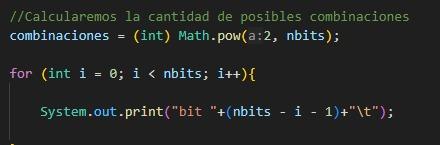
\includegraphics[width=0.5\linewidth]{./latex_imagenes/Img_ejer6_2.jpg}  \\
    -La imprime \\
    \centering
    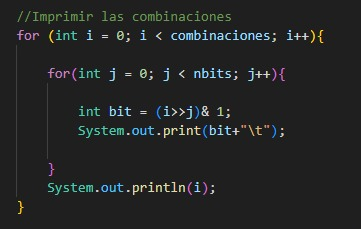
\includegraphics[width=0.5\linewidth]{./latex_imagenes/Img_ejer6_3.jpg}  \\
    -Ingresa la cantidad de salidas que desea tener
    \centering
    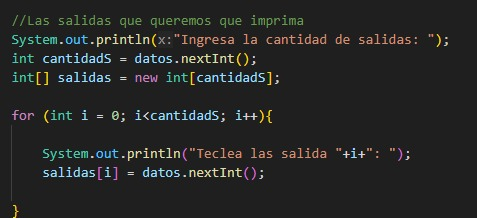
\includegraphics[width=0.5\linewidth]{./latex_imagenes/Img_ejer6_4.jpg}  \\
    - Y con eso se genera la expreción booleana
    \centering
    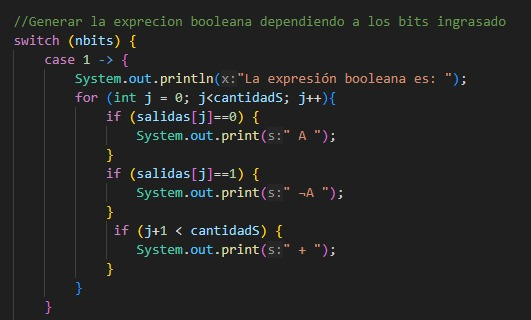
\includegraphics[width=0.5\linewidth]{./latex_imagenes/Img_ejer6_5.jpg}  \\
    

    Depuración de pruebas:

    -Con un bit y dos salidas
    \centering
    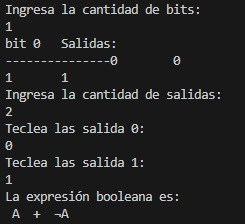
\includegraphics[width=0.5\linewidth]{./latex_imagenes/Img_ejer6_7.jpg}  \\
    -Con dos bits y 3 salidas
    \centering
    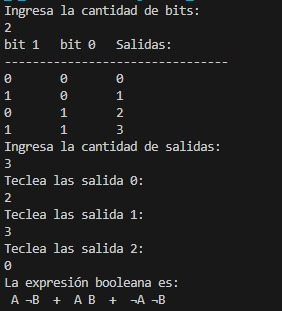
\includegraphics[width=0.5\linewidth]{./latex_imagenes/Img_ejer6_8.jpg}  \\
    -Con tres bits y 2 salidas
    \centering
    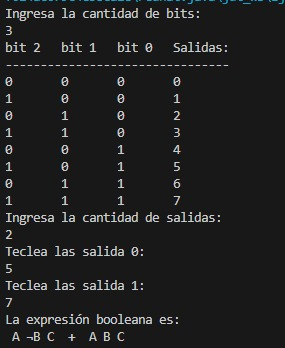
\includegraphics[width=0.5\linewidth]{./latex_imagenes/Img_ejer6_9.jpg}  \\
    -Con cuatro bits y 3 salidas
    \centering
    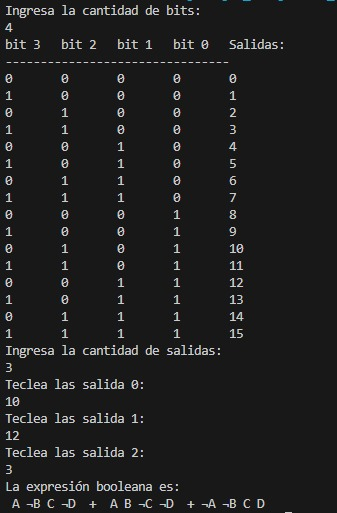
\includegraphics[width=0.5\linewidth]{./latex_imagenes/Img_ejer6_10.jpg}  \\
    


    
    
\end{enumerate}



%\begin{equation}
%y = mx + b.
%\label{eq:recta}
%\end{equation}



\section{CONCLUSION}
En conclusión la realización de los problemas ha revelado que aún falta mucho por descubrir en las matemáticas, un ejemplo de ello son los números complejos aun no se ha hallado la forma de resolver ciertas fórmulas que implican a los números complejos, este trabajo nos dio la oportunidad de conocer el por que de las fórmulas al investigar sus teoremas, el por que de los resultados. Se puede definir que como equipo falta conocer muchas cosas, y que siendo estudiantes aun queda un camino por recorrer para tener un mayor dominio de estas, al igual que aprendimos que las matemáticas son muy útiles, y que son necesarias para conocer, aprender y analizar
\vspace*{-8pt}


\section{AGRADECIMIENTOS}
Agradecemos a losa todos esos maestros que se preocuparon y nos apoyaron en cada paso y también agradecemos a las personas que nos brindaron su ayuda y nos estuvieron apoyando.



\begin{IEEEbiography}{Leilany Aislinn Sánchez Reyes}{\,} Es un estudiante de la ingeniería en Tecnologías de la Información  sus aspiraciones es acabar la carrera a cumplir todos sus sueños tiene una fascinación por los libros y  por bailar y su sueño es ser alguien importante que deje su huella en este mundo para poder ayudar a la gente que más lo necesita poder cambiar al mundo es una estudiante que simpre da lo mejor de sí aunque le cueste.
Pagina de Githud: \url{https://github.com/23Leilany166}
\end{IEEEbiography}

\begin{IEEEbiography}{Rosario Reyes Martinez}{\,} Es un estudiante de la carrera de ingenieria en TICs, sus pasatiempos son leer libros, escuchar musica, al igual que ver series, algunas de sus aspiraciones son terminar la carrera, y en un punto de su vida escribir un libro. 
Pagina de Githud: \url{https://github.com/RosarioReyesMtz}
\end{IEEEbiography}

\begin{IEEEbiography}{Asael Manuel Otero Reyes}{\,} Tiene actualmente 18 años, estudia en el Instituto Tecnológico Superior del Occidente del Estado de Hidalgo (ITSOEH), Es originario del municipio de Francisco I. Madero en el estado de Hidalgo, su objetivo es lograr terminar una carrera y poder valerse por mí mismo.
Pagina de Githud: \url{https://github.com/asaelitop}
\end{IEEEbiography}

\section{REFERENCIAS}

\begin{itemize}
    \item Resolviendo ecuaciones cuadráticas usando la fórmula cuadrática (S.f). En Monterey Institute for Technology and Education (MITE). Recuperado de Torres, C. (S.f). Ecuaciones Cuadráticas. En Investigación en Educación Matemática, Edumate Perú. Recuperado de \url{https://edumate.files.wordpress.com/2008/12/ecuaciones-cuadraticas.pdf} (septiembre, 2015).
\end{itemize}

\begin{thebibliography}{99}
\bibitem{origen_formula}
Instituto de Ciencias Matemáticas. (2014, 22 de mayo). El origen de la fórmula de la ecuación de segundo grado. Blogs Madrid. Matemáticas y sus fronteras. Recuperado de \url{http://www.madrimasd.org/blogs/matematicas/2014/05/22/138152} (septiembre, 2015).

\bibitem{rosen}
Rosen, K. H. (2018). \textit{Discrete Mathematics and Its Applications}. McGraw-Hill Education.

\bibitem{johnsonbaugh}
Johnsonbaugh, R. (2017). \textit{Discrete Mathematics}. Pearson.

\bibitem{kenneth}
Rosen, K. H. (2018). \textit{Elementary Number Theory and Its Applications}. Addison-Wesley.
\end{thebibliography}

Acerca de los números complejos: \url{https://www.uv.mx/personal/aherrera/files/2014/08/01a.-INTRODUCCION-A-LOS-NUMEROS-COMPLEJOS.pdf}.

Puedes visitar la página en el siguiente enlace acerca de los números reales: \url{https://www.mat.uson.mx/~jldiaz/NReales/1-N%C3%BAmeros_Reales.htm}.

El artículo sobre lógica proposicional en la Enciclopedia Stanford de Filosofía proporciona una perspectiva detallada \url{https://plato.stanford.edu/entries/logic-propositional/}









\end{document}

